\chapter{Our traffic scheduler}
\label{chap02}
%motivation: little config (knobless), fast O(1), QoS aware, scheduler in presence of differentiated services. Would run at simple devices

\begin{figure}
	\centering
	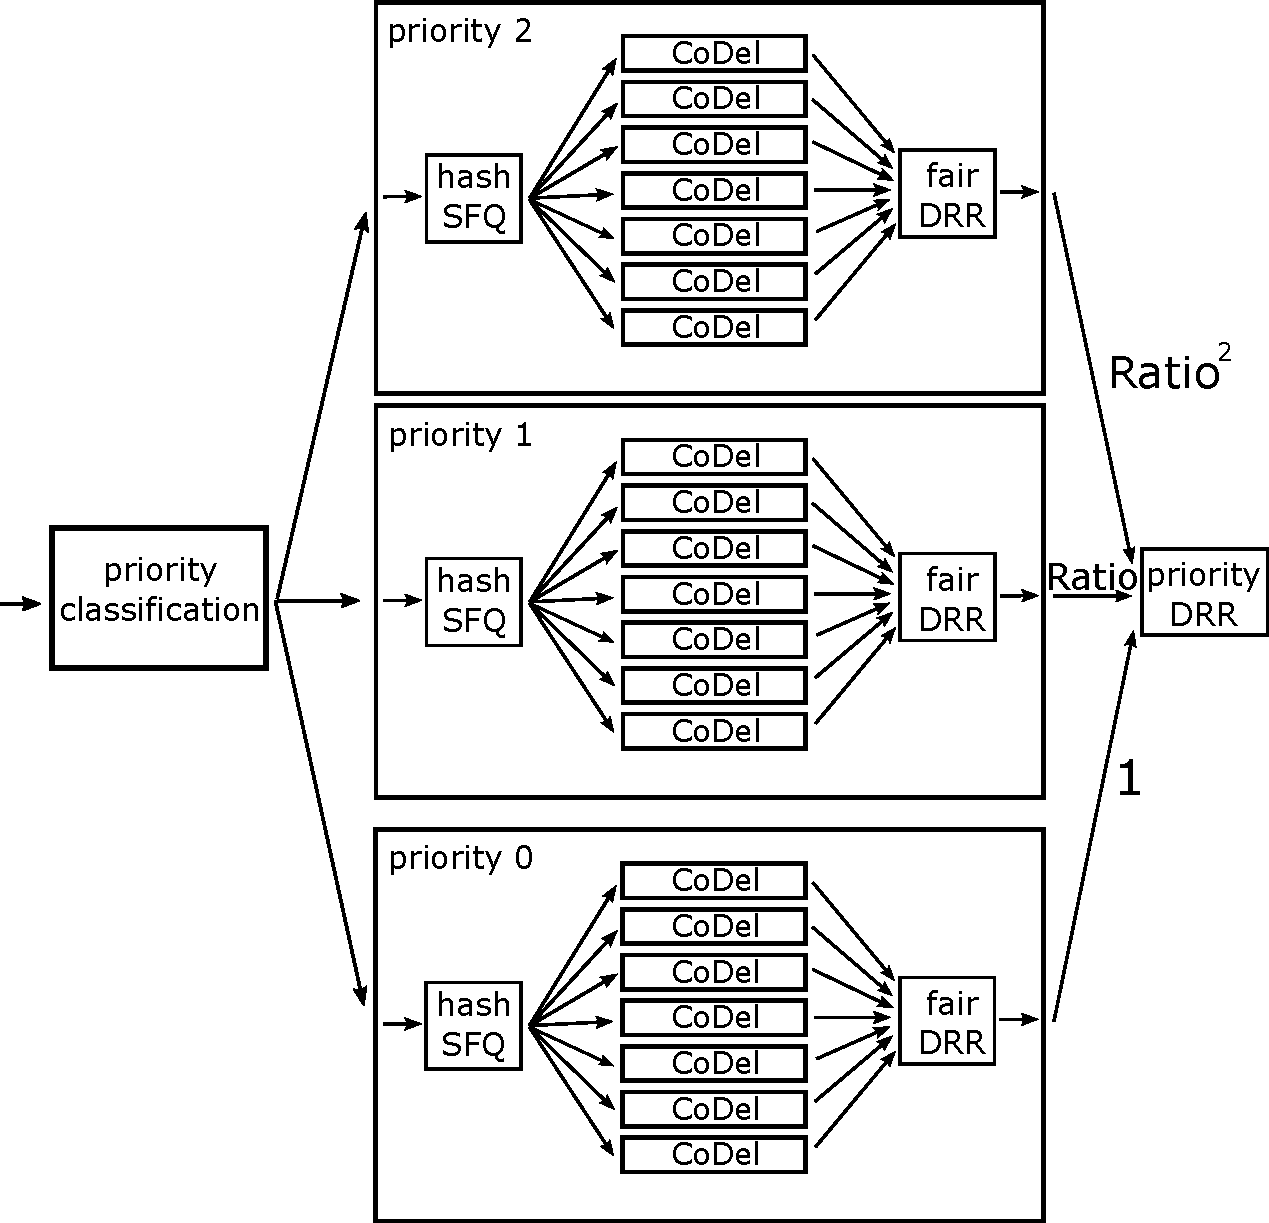
\includegraphics[width=137mm]{drawings/msfc}
	\caption{The MSFC layout}
	\label{fig10:msfc}
\end{figure}

In this thesis, we propose a traffic scheduler Multilevel stochastic fairness queueing (MSFC) illustrated in \ref{fig10:msfc}. It combines ideas of previous work: CoDel and deficit round-robin, to create classful traffic scheduler. It uses three-level layout. In the highest level, packets are assigned to priority classes. We use non-fair DRR to prioritize more important traffic. Inside the classes, packets are distributed into flows (based on source and destination IP addresses, ports and protocol) and we use second, independent fair DRR to schedule traffic within the class. Each flow uses CoDel algorithm.

. 

Additionally, it has following parameters:
\begin{itemize}
	\item $Limit$ --- the maximum amount of packets stored in the qdisc.
	\item $Prios$ --- the number of priority classes (max 8).
	\item $Flows$ --- the number of queues (CoDels) in each priority class (so there is $Prios*Flows$ total independent CoDels)
	\item $Backlog$ --- the maximum backlogged bytes in an individual CoDel.
	\item $Perturb$ --- number of seconds after flow-classification hash function perturbs
	\item $Quantum$ --- the quantum parameter of the inner fair DRR (see \ref{DRR})
	\item $Target$ --- target delay parameter for CoDel algorithm (see \ref{CoDel})
	\item $Interval$ --- Interval parameter for CoDel algorithm (see \ref{CoDel})
	\item $Ratio$ --- defines the ratio of bandwidth of two adjacent priority classes. The ratio is enforced by the outer DRR. MSFC uses $Ratio$ to compute quantums of all priority classes. The quantums rise exponentially:
	\[
	Q_p = Quantum \cdot Ratio^p,
	\]
	where $p$ is the priority of class, and $Quantum$ is the parameter for inner DRR.
\end{itemize}
So if there are 3 classes with priorities 0--2 (like in the Figure \ref{fig10:msfc}), the upstream bandwidth will be distributed in ratio $1:Ratio:Ratio^2$.

Note, that the ratio is independent of the number of flows in each class. Consider two classes with adjacent priorities 0 and 1. Priority 1 class has only one flow backlogged, priority 0 class has 100 flows. The one flow from priority 1 class is guaranteed to receive 2/3 of the bandwidth. The 1/3 is distributed fairly between the remaining 100 flows.

\section {Implementation}

We have implemented the algorithm into Linux kernel. 

In Linux IP/MPLS routers, traffic flows are controlled by
three kinds of objects: qdiscs (queuing disciplines), classes and
filters [7-11]. Queueing discipline (qdisc) controls the packet
scheduling for a specific network interface. Whenever the
kernel needs to send a packet to an interface, it enqueues the
packet to the qdisc configured for the interface. Immediately
afterwards, the kernel tries to get as many packets as possible
from the qdisc for giving them to the network adaptor driver.
Some qdiscs can contain classes which contain further
inner qdiscs; traffic may then be enqueued in any of the inner
qdiscs, which are within the classes. When the kernel tries to
dequeue a packet from such a classful qdisc, it can come from
any of the classes. A qdisc may for example prioritize certain
kinds of traffic by trying to dequeue from certain classes before
others.
Filter is used by a classful qdisc to determine in which
class a packet will be enqueued. Whenever a traffic arrives at a
class with subclasses, it needs to be classified. All filters
attached to the class are called until one of them returns with a
verdict. Filters reside within qdiscs.
Even though the traffic control components in Linux kernel
are partially implemented, the traffic control for QoSguaranteed
DiffServ provisioning with optimized bandwidth
sharing and priority-based preemption has not evaluated and
confirmed in depth. Especially, to the best knowledge of
authors, the comparisons with different combinations of qdisc,
class and filter have not been reported yet.


-ns3 --- seeds and replication of results

skombinovanie CoDel + SFQ + DRR + QoS


